% Springer LNCS template (llncs.cls v2.26)
\documentclass[runningheads]{llncs}

\usepackage[T1]{fontenc}
\usepackage[utf8]{inputenc}
\usepackage{lmodern}
\usepackage{graphicx}
\usepackage[notransparent]{svg}
\svgpath{{figures/svg/}}
\svgsetup{inkscapepath=svgsubdir}
\usepackage{xcolor}
\usepackage{microtype}
\usepackage{booktabs}
\usepackage{tabularx}
\usepackage{array}
\usepackage{cite}
\usepackage{url}
\usepackage[hidelinks]{hyperref}
\renewcommand\UrlFont{\color{blue}\rmfamily}
\urlstyle{rm}

\begin{document}

\title{Designing a National Student Innovation Challenge: Insights from an Experiential Learning Programme in India}
\titlerunning{Designing a National Student Innovation Challenge}

% TODO: add authors and affiliations
\author{}
% \author{First Author\inst{1}\orcidID{0000-0000-0000-0000} \and
% Second Author\inst{1}}
% \authorrunning{F. Author et al.}
\institute{}
% \institute{e-Yantra, Indian Institute of Technology Bombay, Mumbai, India\\
% \email{...}}

\maketitle

\begin{abstract}
Higher education in India often lacks structured pathways for students to move from classroom learning to building real-world, deployable solutions. This experience report presents a national student e-Yantra innovation challenge(eYIC) hosted by a premier institute in Bombay, India, that addresses this gap by engaging student teams in identifying real-world problems and developing technology-based solutions through structured mentoring and staged evaluation. The participating teams consisted of two to four student members each with varied backgrounds ranging from engineering to science. The challenge applies established ideas from experiential and project-based learning with expert mentorship, and self-paced online learning in the setting of an interdisciplinary national challenge open to students across degree programmes. This report presents insights from the 2025-26 cycle, themed around Agriculture. The programme followed a multi-stage model consisting of ideation, mentored prototyping, technical evaluation, and final pitching. It combined regional ideation workshops, online and offline mentoring, technical and entrepreneurship MOOCs, periodic progress reviews, and travel and component reimbursements for participating teams. Of 323 registered teams, 290 submitted proposals, 149 advanced to the mentored sprint stage, 33 reached the Regional Finals, and 16 reached the Finals. Participant feedback was strongly positive, with Regional Finals participants reporting an overall satisfaction score of 4.81/5, while the mentored sprint stage and mentorship were rated 4.53/5 and 4.40/5 respectively. At the same time, the programme surfaced major participant challenges of compressed timelines, access to field visits, identifying and addressing authentic problems, and access to local knowledge. We connect these challenges to adoptable responses, including protecting field-study time, assigning dedicated per-team mentors, strengthening onboarding to MOOCs, and adding regional centres. Our insights suggest that staged mentorship, experiential problem-finding, and interdisciplinary idea-to-product scaffolding can support student innovation pathways. The report offers practical guidance for institutions seeking to design and implement similar interdisciplinary innovation challenges in higher education.

\sloppy
\keywords{Innovation challenge \and Project-based learning \and Entrepreneurship \and Sustainability \and Agriculture \and Experiential learning \and Mentorship \and Interdisciplinary education}
\end{abstract}



\section{Introduction}

Higher education institutions are increasingly expected to prepare students not only with disciplinary knowledge, but also with the ability to identify real-world problems, collaborate across disciplinary boundaries, and develop innovative solutions with societal relevance \cite{b1}, \cite{b2}. Although universities provide strong foundations in domain-specific knowledge, students may receive limited opportunities to engage in authentic problem identification, stakeholder interaction, user-centred design, prototyping, and iterative solution development \cite{b3}. Consequently, many students complete their formal education without experiencing the complete process of translating an observed societal need into a contextualised and practically viable solution.

Experiential learning \cite{b4}, \cite{b5} and project-based learning \cite{b6}-\cite{b8} have been widely recognised as effective pedagogical approaches for developing competencies such as critical thinking, creativity, teamwork, communication, and problem solving. Innovation-oriented learning programmes extend these approaches by asking students to investigate real contexts, engage with stakeholders, question their initial assumptions, generate alternative ideas, and repeatedly refine their solutions through feedback and testing \cite{b9,b10,b11}. Such programmes can create opportunities for students to learn through the uncertainties, negotiations, and failures that characterise authentic innovation practice rather than through predetermined classroom exercises alone.

However, enabling such experiences at scale presents several pedagogical and operational challenges. Student teams may enter innovation programmes with varying levels of technical knowledge, design experience, disciplinary preparation, and familiarity with real-world problem investigation. Interdisciplinary teams must learn to integrate different forms of expertise while developing a shared understanding of the problem and the proposed solution \cite{b13}. Participants also require sustained mentorship to move from broad ideas to clearly articulated problems, feasible prototypes, and evidence-informed claims about potential impact \cite{b12}. At a national level, these challenges are compounded by geographical distribution, differences in institutional infrastructure, uneven access to domain experts, and the need to evaluate both the process and outcomes of innovation consistently.

The eYIC was conceptualised in response to these concerns as a structured national programme through which interdisciplinary student teams could progress from identifying authentic societal problems to developing and presenting technology-enabled solutions. The programme is open to students from diverse academic backgrounds, including engineering, science, arts, management, and other disciplines. This interdisciplinary orientation is based on the premise that meaningful innovation emerges through the integration of multiple perspectives rather than through technical expertise alone \cite{b13}. The programme therefore positions innovation as a collaborative and iterative process involving problem identification, contextual inquiry, stakeholder engagement, ideation, prototyping, validation, and communication \cite{b9,b10,b11}.

The programme was guided by three central premises. First, the quality of an innovation depends on the team’s understanding of the problem and its context, rather than only on the sophistication of the final prototype. Second, interdisciplinary participation can broaden how problems are interpreted and enable teams to consider technical, social, economic, and user-related dimensions of proposed solutions \cite{b13}. Third, students require progressive scaffolding, mentoring, and repeated feedback to navigate the movement from an initial idea to a feasible and contextually grounded innovation \cite{b12}. Accordingly, the programme combines contextual problem investigation, structured learning resources, expert-led workshops, regular mentorship, iterative prototype reviews, and multi-stage evaluations. Teams are evaluated not only on their final artefacts but across successive stages: during the sprints, on problem validation, the practicality and feasibility of their solutions, the alignment of team skills with the required technology, and implementation progress; and at the Grand Finale, on innovation, technical excellence, social impact, entrepreneurial potential, and presentation.

\begin{figure}[htbp]
\centering
\includesvg[width=\textwidth,inkscapelatex=false]{image1}
\caption{Conceptual framework of the eYIC, showing how the three guiding premises inform programme design and the criteria on which teams are evaluated.}
\label{fig1}
\end{figure}

This experience report describes the design and implementation of the 2025-26 edition of the programme of the eYIC. It examines how the programme supported interdisciplinary student teams across successive stages of problem identification, solution development, mentorship, evaluation, and pitching. The report also documents the programme structures that enabled national-level implementation, the experiences of participating teams and programme stakeholders, and the practical challenges encountered during delivery. By presenting both the strengths and limitations of the programme, the paper offers design considerations for higher education institutions and organisations seeking to implement scalable, mentorship-supported innovation programmes for geographically and disciplinarily diverse student populations.

\section{Related Work}

Experiential learning provides an important pedagogical basis for programmes that engage students in addressing authentic problems. In this tradition, learning develops through recurring cycles of concrete experience, reflection, conceptualisation, and experimentation \cite{b4}\cite{b5}\cite{b14}. Project-based learning operationalises these principles by organising learning around sustained investigations in which students address meaningful problems and develop tangible artefacts \cite{b15}. Comparative studies indicate that project-based learning can support the application and longer-term retention of knowledge more effectively than conventional instruction \cite{b16}. Studies in engineering education similarly associate project-based learning with the development of problem-solving, teamwork, communication, and self-directed learning competencies \cite{b17}, \cite{b18}. At the same time, the literature identifies recurring challenges related to student workload, assessment, facilitation, and the integration of knowledge across disciplines \cite{b17}, \cite{b18}. These findings suggest that authentic projects alone may not be sufficient; students also require structured milestones, feedback, and support throughout the project lifecycle.

Innovation challenges, hackathons, and design competitions provide another context in which experiential and project-based learning are enacted. Educational hackathons typically bring participants together to identify problems, generate ideas, build prototypes, and present solutions within an intensive and time-bounded collaborative setting \cite{b19}, \cite{b20}. Reviews of such initiatives report positive outcomes related to engagement, teamwork, skill acquisition, creativity, and rapid problem solving, while also identifying difficulties associated with limited time, unequal participant preparation, resource availability, and integration with formal educational structures \cite{b19}. More recent studies conceptualise hackathons as experiential learning environments in which participants develop engineering-design and problem-solving competencies under conditions of uncertainty and time pressure \cite{b21}. However, the compressed duration of many hackathons may constrain opportunities for sustained stakeholder engagement, problem validation, iterative testing, and the development of technically and contextually mature solutions.

Competition-based learning extends some of these principles by organising project activity around sequential tasks, milestones, feedback, and performance-based progression. Rather than treating competition only as a mechanism for ranking participants, educational competitions can use challenge structures to sustain participation, create meaningful deadlines, and provide a shared context for applying disciplinary knowledge. In India, large-scale robotics competitions have demonstrated how project-based learning can be delivered to geographically distributed student teams through online resources, structured tasks, hardware-based activities, and successive stages of evaluation \cite{b30}, \cite{b31}. Related studies have examined participation in resource-constrained settings, inclusiveness, learner progression, and dropout in such competition-based models \cite{b32,b33,b34}. These initiatives demonstrate the potential of staged competitions to support experiential learning at scale, while also revealing the need for carefully designed scaffolding and sustained participant support.

Mentorship is particularly important in programmes where students are expected to work on unfamiliar, interdisciplinary, and open-ended problems. Formal mentorship programmes in higher education have been associated with increased career self-efficacy, a stronger sense of institutional connection, and improved academic and professional development \cite{b22}, \cite{b23}. Mentors can help participants clarify goals, examine assumptions, access relevant expertise, interpret feedback, and sustain progress during periods of uncertainty. Within innovation programmes, mentorship may also serve as a bridge between broad ideas and implementable solutions by supporting teams in problem formulation, stakeholder engagement, technical development, and validation. Nevertheless, the effectiveness of mentorship depends on the suitability of mentor–team matching, the regularity of interaction, clarity of expectations, and continuity of support. These concerns are especially significant in national programmes involving large numbers of teams and mentors with different forms of disciplinary and professional expertise.

The use of self-paced online learning further enables innovation programmes to provide technical and entrepreneurship-related resources to geographically distributed participants. Massive open online courses and similar online learning environments can expand access to specialised content, but frequently experience low completion and retention when learners engage without facilitation, interaction, or feedback \cite{b24}. Blended approaches that combine self-paced content with mentoring, collaborative activity, periodic reviews, or face-to-face engagement have been found to improve participation and persistence relative to purely online delivery \cite{b25}. This literature supports positioning online courses as one component within a broader learning arrangement rather than as an independent intervention. In innovation challenges, online resources may provide foundational knowledge, while mentoring and project milestones help teams interpret and apply that knowledge to their specific problems.

Interdisciplinary education is also central to programmes that address complex societal challenges. Such problems often involve interconnected technical, social, economic, environmental, and user-related considerations that cannot be adequately addressed from a single disciplinary perspective. Interdisciplinary learning can support students in integrating different forms of knowledge, negotiating alternative interpretations, and developing more comprehensive responses to real-world problems \cite{b26}. However, interdisciplinary teamwork also presents challenges because team members may use different vocabularies, methods, assumptions, and criteria for evaluating solutions. Programme structures must therefore support not only the division of tasks among students from different disciplines, but also the development of shared problem understanding and integrated solutions.

These concerns are particularly relevant in the Indian higher education context. Reports on graduate employability have repeatedly pointed to gaps between formal disciplinary preparation and the competencies expected in professional practice \cite{b27}, \cite{b28}. The National Education Policy 2020 similarly emphasises multidisciplinary education, experiential learning, creativity, innovation, and the development of practical and professional capabilities \cite{b29}. Competition-based and project-based initiatives have emerged as one response to these priorities, particularly in engineering and technology education. However, many established competition models begin with prescribed technical problems or predetermined artefacts. They provide valuable opportunities for implementation and technical problem solving but may offer less emphasis on the preceding processes of contextual inquiry, stakeholder engagement, open-ended problem identification, and validation of societal need.

The eYIC reported in this paper integrates experiential and project-based learning, mentorship, blended learning, interdisciplinarity, and competition-based learning within a multi-month, staged programme. Unlike short-duration hackathons or competitions built around predefined technical tasks, it supports interdisciplinary teams in identifying problems, engaging stakeholders, developing and refining technology-enabled solutions, and presenting them through regional and national evaluations. This experience report addresses the limited documentation of how these components can be orchestrated at national scale by examining the programme’s design, implementation, and practical tensions across the idea-to-solution journey in agriculture.

\section{Theoretical Grounding}

The Innovation Challenge is grounded in experiential learning, situated cognition, cognitive apprenticeship, and social interdependence. Together, these perspectives explain how students learn through authentic problem engagement, iterative solution development, expert guidance, and interdisciplinary collaboration. Experiential Learning Theory conceptualises learning as a recurring movement among concrete experience, reflective observation, abstract conceptualisation, and active experimentation \cite{b14,b15,b16}. In the Innovation Challenge, concrete experience begins with investigating problems in real-world settings and interacting with relevant stakeholders. Workshops, self-paced courses, and expert sessions help teams connect these experiences with conceptual and technical knowledge. Mentor feedback and periodic reviews create opportunities for reflection, while prototyping, testing, and redesign enable teams to actively experiment with their emerging ideas. The programme therefore treats innovation not as the production of a single final artefact, but as an iterative learning process in which problem understanding and proposed solutions evolve together.

Situated cognition further emphasises that knowledge cannot be separated from the activities, contexts, and communities in which it is developed and used \cite{b35}. From this perspective, learning to innovate requires more than acquiring generic technical or entrepreneurial knowledge. Students must learn to interpret local practices, stakeholder needs, material conditions, and constraints within the contexts where their solutions are intended to function. The programme’s emphasis on field investigation and stakeholder engagement therefore situates student learning within authentic agricultural contexts rather than presenting innovation as a decontextualised classroom exercise. This grounding also explains why problem validation and contextual relevance are considered alongside technical implementation during evaluation. Cognitive apprenticeship provides a basis for understanding the role of mentorship and staged support within the programme \cite{b36}. In cognitive apprenticeship, experts make otherwise tacit processes visible through modelling, coaching, scaffolding, articulation, reflection, and guided exploration. Within the Innovation Challenge, workshops and learning resources introduce processes such as problem framing, stakeholder inquiry, design, prototyping, validation, and pitching. Mentors and domain experts subsequently coach teams as they apply these processes to their own projects, question assumptions, diagnose difficulties, and refine their decisions. Successive milestones and reviews provide temporary structures that support teams during complex stages while progressively encouraging greater ownership of problem-solving and solution development.

Adding to the above theoretical standpoints, the Social Interdependence Theory proposes that productive cooperation develops when participants perceive that their goals are connected and that successful outcomes depend on coordinated contributions \cite{b37}. Interdisciplinary grouping alone may therefore be insufficient; teams also require shared goals, complementary responsibilities, interaction, and mutual accountability. Within the challenge, collective project milestones, prototype development, reviews, and team-based presentations create conditions in which students must integrate technical, social, managerial, and contextual perspectives. Collaboration becomes not merely a division of tasks, but a process of negotiating different forms of knowledge to develop a coherent problem understanding and solution.

Taken together, these perspectives frame the Innovation Challenge as a situated and progressively scaffolded learning environment. Experiential learning explains the iterative movement between action, reflection, conceptual understanding, and experimentation; situated cognition foregrounds authentic contexts and stakeholder practices; cognitive apprenticeship explains the role of mentors, resources, and staged reviews; and social interdependence highlights the collaborative work required within interdisciplinary teams. The competition structure provides the temporal and evaluative architecture through which these processes are organised, supporting teams as they move from contextual problem identification to the development, validation, and communication of technology-enabled solutions.

\section{Design of eYIC}

The design of the eYIC translates the pedagogical principles discussed earlier into a staged programme through which student teams progressively move from identifying a real-world problem to developing, demonstrating, and communicating a functional solution. Rather than treating the challenge as a single competition event, the programme is organised as a six- to seven-month learning journey combining problem identification, self-paced learning, mentorship, prototype development, iterative evaluation, and pitching. The 2025–26 edition was organised around the broad domain of agriculture and involved teams of two to four students from engineering and science disciplines. The programme design comprises three interconnected elements: (1) the phase-wise progression of teams, (2) the mentorship and resource infrastructure supporting this progression, and (3) staged evaluation criteria that change as teams move from problem understanding towards product development. The figure below  presents the overall programme timeline and learning architecture.

\subsection{Phase-Wise Progression}

The programme begins with an ideation and problem-identification stage (see Fig.~\ref{fig2}). Student teams register under the broad thematic domain and are encouraged to identify problems that emerge from actual contexts rather than beginning with predetermined technical solutions. Regional ideation workshops support this process through guided problem exploration, while teams are encouraged to undertake field visits and interact with relevant stakeholders to understand local practices, constraints, and needs. Teams subsequently articulate their identified problem and proposed direction through a formal proposal. In the 2025–26 edition, 323 teams registered for the challenge, of which 290 submitted proposals.

\begin{figure}[htbp]
\centering
\includesvg[width=0.8\textwidth,inkscapelatex=false]{image2}
\caption{Programme timeline of the 2025–26 edition, showing sequential stages and the learning resources released in parallel with them.}
\label{fig2}
\end{figure}

Following proposal screening, selected teams enter the implementation and mentorship stage (see Fig.~\ref{fig2}), organised through a series of development sprints. A total of 149 teams progressed to this stage. The initial sprint focuses on translating the proposed idea into a feasible system architecture, including decisions related to hardware, software, component selection, and overall design. Subsequent sprints support teams in integrating individual modules and moving from early-stage concepts or benchtop prototypes towards functional systems. Reviews are conducted periodically, enabling teams to present their progress, receive feedback, identify implementation difficulties, and revise their solutions before proceeding further.

The programme combines online and in-person experiences across these development stages. As shown in Fig.~\ref{fig2}, the first Impulse Sprint is conducted online, followed by an offline second sprint and a third sprint that combines online interaction with mentor review. Technical MOOCs are released alongside the first Impulse Sprint rather than functioning as a separate course sequence, allowing teams to access relevant knowledge while developing their projects.

Teams demonstrating sufficient progress subsequently enter the product-development and showcase stage (see Fig.~\ref{fig2}). Thirty-three teams qualified for the Regional Finals, where they presented working hardware and software prototypes. From these, 16 teams progressed to the Grand Finale. At these final stages, teams are expected not only to demonstrate the functionality of their prototypes but also to articulate the relevance, feasibility, cost considerations, potential deployment, and broader value of their solutions to panels comprising academic, industry, and domain experts. Progression through the programme thus involves a gradual shift in emphasis: from understanding and validating the problem, to developing and integrating a technical solution, and eventually to demonstrating a viable product and communicating its potential for deployment. The staged evaluation criteria summarised in Table~\ref{tab1} reflect this movement from ``problem understanding'' towards ``product synthesis.'' Fig.~\ref{fig3} illustrates activities from three stages of the 2025–26 edition: ideation workshops and prototype demonstrations at the Grand Finale.

\begin{figure}[htbp]
\centering
\includesvg[width=0.75\textwidth,inkscapelatex=false]{image3}
\caption{Participant activities in the 2025–26 edition: (a) teams engaged in group problem-exploration activities during a regional ideation workshop; (b) working prototypes presented at the Grand Finale.}
\label{fig3}
\end{figure}

\subsection{Learning, Mentorship, and Resource Support}

To support teams from heterogeneous educational and institutional backgrounds, the challenge combines mentorship, self-paced learning, and logistical support throughout the programme. These components operate alongside the staged project activities rather than as independent interventions. Mentorship provides teams with recurring opportunities to discuss their ideas and prototypes with technical mentors, domain experts, and reviewers. Mentoring is particularly important during the sprint stages, where teams encounter decisions relating to system architecture, component selection, integration, implementation, and troubleshooting. Periodic mentor reviews serve both as developmental checkpoints and as opportunities for teams to reconsider assumptions and refine their solutions. As shown in Fig.~\ref{fig2}, innovation and entrepreneurship learning resources are introduced during the ideation stage, while technical MOOCs are offered during the implementation and mentorship stage. This sequencing is intended to provide teams with relevant learning resources at the stage where they can apply them to their projects.

The technical MOOCs are designed to provide exposure to the core technology domains, such as ROS, embedded systems, software foundations, drones, and related technologies. These MOOCs focus on building a foundational technical skill set and are not necessarily aligned with or limited to the specific domain chosen for a team's project.

A third component is logistical and financial scaffolding. Since teams participate from institutions distributed across different regions, participation can be constrained by access to hardware, components, and travel. The programme therefore provides component reimbursements to eligible teams during prototype development and travel support for teams progressing to Regional Finals and Grand Finale. These mechanisms are intended to reduce resource-related barriers to continued participation. Together, these structures create a distributed support system in which learning resources provide foundational knowledge, mentors support contextual application and troubleshooting, and financial and logistical provisions enable teams to continue developing and presenting their solutions.

\subsection{Staged Evaluation and Progression}

Evaluation is integrated throughout the challenge rather than being restricted to assessment of the final prototype. The criteria evolve alongside the expected development of the teams, allowing different dimensions of innovation to become salient at different stages (Table~\ref{tab1}). During the ideation and proposal stage, evaluation primarily considers whether the identified problem lies within the agriculture domain and has been appropriately validated, the practicality and feasibility of the proposed solution, and the technical readiness of the proposal, including the relevance of hardware and software specifications, the alignment of team skills with the required technology, and the reasonableness of the proposed timeline. Since problem validation requires teams to substantiate their problem through field visits and interactions with stakeholders, it also serves as an indirect measure of stakeholder engagement and field grounding. At this stage, emphasis is placed on whether teams have sufficiently understood the problem before committing to a technical response.

During the Impulse Sprints, attention shifts towards the development of the proposed system. The first sprint assesses the extent of implementation completed and the likelihood of completion within the stipulated time, while the second is entirely formative, with evaluators providing only remarks and suggestions. The third sprint applies the most detailed technical rubric of the programme, covering system architecture and design clarity, implementation progress, technology stack, algorithm or model implementation, testing, validation status, feasibility of the current build, and progress since the previous review. Feedback during these reviews enables teams to identify gaps and refine their prototypes before subsequent stages.

Progression to the Regional Finals is determined through a technical video submission, on the basis of which evaluators recommend whether teams should advance. Selection for the Grand Finale is then made through offline evaluation informed by evaluator remarks and the technical video. At the Grand Finale, evaluation moves from technical progress towards the value of the solution, with award categories assessing innovation, technical excellence, social impact, entrepreneurial potential, and the quality of the business pitch, including customer discovery, market and competitor analysis, and pricing. The changing criteria therefore parallel the programme's progression from problem understanding towards product synthesis rather than applying an identical assessment framework throughout the challenge.

\begin{table}[htbp]
\centering
\caption{Stage-wise evaluation focus and criteria in the 2025–26 edition}
\label{tab1}
\scriptsize
\renewcommand{\arraystretch}{1.2}
\begin{tabularx}{\textwidth}{@{}>{\raggedright\arraybackslash}p{0.17\textwidth}>{\raggedright\arraybackslash}p{0.17\textwidth}>{\raggedright\arraybackslash}X>{\raggedright\arraybackslash}p{0.17\textwidth}@{}}
\toprule
\textbf{Stage} & \textbf{Evaluation focus} & \textbf{Key criteria} & \textbf{Outcome} \\
\midrule
Ideation Sprint & Problem grounding and proposal quality & Agriculture-domain problem; problem validation (reflecting field and stakeholder engagement); practicality and feasibility; technical specifications; team skill alignment; block diagrams; timeline & Shortlisting; mentor interest; suggestions \\
Impulse Sprint 1 (online) & Implementation progress & Extent completed; likelihood of timely completion; finalist potential & Progression judgement; suggestions \\
Impulse Sprint 2 (offline) & Formative feedback & Open remarks only & Written suggestions \\
Impulse Sprint 3 (online) & Technical rigour & Architecture; implementation; technology stack; algorithm/model; testing; validation; feasibility; progress since last review & Scored technical review \\
Technical video & Readiness to advance & Advance recommendation; reserve consideration; comments & Selection for Regional Finals \\
Regional Finals & Selection for Grand Finale & Offline evaluation using remarks and video & 16 of 33 teams selected \\
Grand Finale & Product synthesis and value & Innovation; technical excellence; social impact; entrepreneurial potential; business pitch (1–5 scales) & Category awards \\
\bottomrule
\end{tabularx}
\end{table}

\section{Methods}

\subsection{Participants and Programme Context}

This experience report draws on the 2025-26 implementation of eYIC, organised around the broad thematic domain of agriculture. Students participated in teams of two to four and progressed through successive stages of problem identification, proposal development, mentored prototyping, regional evaluation, and the national finale. A total of 323 teams registered for the programme, of which 290 submitted formal proposals. Following proposal review and shortlisting, 149 teams progressed to the mentored prototyping and Impulse Sprint stage. Subsequent evaluations resulted in 33 teams participating in the Regional Finals, from which 16 teams were selected for the Grand Finale. The programme therefore provides an opportunity to examine participant experiences across different stages of an extended national innovation journey rather than at a single competition event.

\subsection{Data Sources}

The experience report draws on multiple sources of programme-generated data collected during the implementation of eYIC. These include registration and team-progression records, submitted proposals, records from the Impulse Sprints and periodic reviews, evaluation rubrics from successive stages, and participant feedback collected during or after the programme. Programme records were used to trace team participation and progression across the major stages of eYIC. Proposal and review artefacts provided evidence of how teams moved from initial problem formulations towards prototype development. Evaluation records captured the dimensions emphasised at different stages, including problem understanding and stakeholder grounding during ideation, technical architecture and system integration during the sprint stages, and prototype functionality, feasibility, deployment potential, and pitching during the regional and national finals. Participant feedback was used to understand how students experienced different programme components, including the ideation activities, Impulse Sprints, mentoring, learning resources, evaluation processes, and overall challenge. Where available, reflections and observations from mentors and the programme orchestration team were also considered to identify implementation challenges and adaptations made during the programme.

\subsection{Data Analysis}

A mixed-methods descriptive approach was adopted to examine both programme progression and participant experience. The analysis was organised around three dimensions.First, team progression was examined descriptively by tracing the number of teams participating at each major stage: registration, proposal submission, mentored prototyping, Regional Finals, and Grand Finale. Rather than interpreting progression solely as competition-based elimination, these records were used to understand the different levels of engagement reached by teams within the programme. Second, programme artefacts and evaluation records were examined across successive stages to understand how expectations changed as teams moved through the innovation process. Particular attention was given to the progression from problem identification and stakeholder validation to system development, prototype integration, and final product demonstration. This analysis was aligned with the staged evaluation architecture of eYIC, in which criteria progressively shift from problem understanding towards product synthesis. Third, participant feedback and programme-team reflections were analysed to identify recurring patterns concerning the learning and implementation experience. Quantitative feedback items were summarised using descriptive statistics, while open-ended responses and reflections were reviewed thematically to identify recurring strengths, challenges, and suggestions for programme improvement. The analysis focused particularly on experiences related to mentorship, the Impulse Sprints, learning resources, field engagement and problem validation, evaluation processes, and the overall programme timeline. Together, these analyses were used to examine not only programme reach and progression, but also how different elements of the eYIC design supported or constrained teams as they moved from problem identification towards the development and communication of technology-enabled solutions.

\section{Findings}

\subsection{Progression through the Innovation Journey}

The 2025-26 edition reached 2,376 registered students, with 1,228 paid participants forming 323 teams across 185 colleges. Ninety of these institutions were outside the existing e-Yantra Lab Setup Initiative (eLSI) network, indicating that the programme extended beyond institutions already connected to e-Yantra. Although the challenge was open across disciplines, actual participation remained predominantly engineering-oriented, with Electronics and Communication Engineering and Computer Science and Engineering representing the largest groups. Thus, while eYIC was interdisciplinary in its intended participation model, the realised cohort remained strongly technology-oriented.

The programme began with broad participation and progressively narrowed as teams advanced through increasingly demanding stages of development. Of the 323 registered teams, 290 submitted proposals, after which 149 teams progressed to the Impulse Sprint stage. The programme design subsequently required teams to demonstrate increasing levels of technical maturity; by the later Impulse Sprint, teams were expected to demonstrate a working prototype rather than present an idea or concept alone. Regional and final stages further shifted the emphasis towards integrated prototype performance, deployment considerations, and communication of the proposed solution.

This progression is important because the participant feedback indicates that the nature of learning and difficulty changed alongside these expectations. Early-stage responses predominantly concerned how to identify and structure meaningful problems, whereas later-stage responses increasingly concerned technical implementation, debugging, access to expertise, timelines, resources, and evaluation. Thus, the programme progression represented not only a process of competitive shortlisting but also a shift in what participants were required to learn and accomplish.

\subsection{Early-Stage Scaffolding Supported a Shift towards Problem-First Innovation}

Feedback from the ideation activities was strongly positive (Fig.~\ref{fig4}a). Across the 1,089 workshop responses, the three five-point rating items had means of 4.41, 4.38, and 4.44, with between 85.1\% and 87.1\% of respondents selecting either 4 or 5. This pattern suggests that participants broadly perceived the workshop experience and associated guidance positively. The annual programme report similarly describes the ideation activities as interactive and hands-on, with particular emphasis on problem identification, design thinking, entrepreneurship, and real-world application.

More importantly, the open-ended responses suggest that the value of the early programme lay not simply in participant satisfaction but in how students began to approach innovation problems. An exploratory coding of 434 unique substantive responses concerning the valuable aspects of the innovation stage identified problem identification and problem framing as the most prominent theme, appearing in 164 responses (37.8\%) (Fig.~\ref{fig4}b). This was followed by design thinking and ideation techniques (22.4\%), business and entrepreneurship-related thinking, including the Business Model Canvas (21.0\%), and the value of having a structured process for moving from an idea towards a solution (20.3\%). Confidence and changes in innovation mindset were also evident in participants' reflections.

\begin{figure}[htbp]
\centering
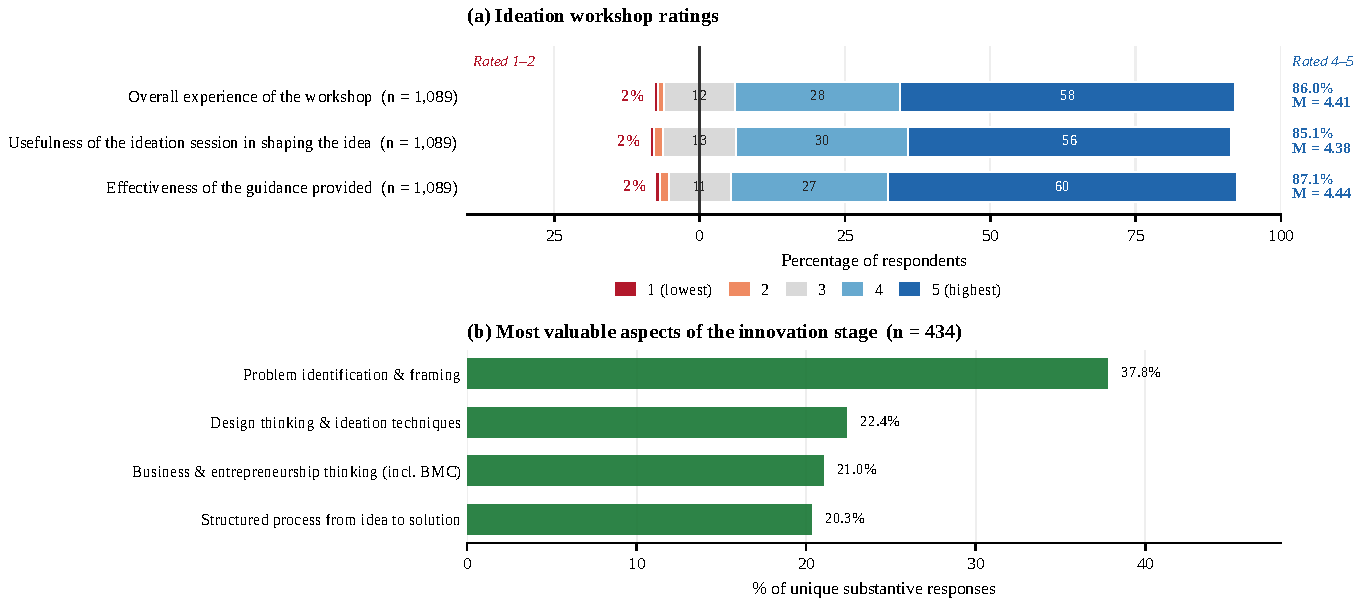
\includegraphics[width=\textwidth]{figures/image4}
\caption{Ideation-stage feedback. (a) Ratings of the ideation workshop (n = 1,089); values on the right give the percentage rating 4–5 and the mean (M). (b) Themes in 434 unique substantive responses on the most valuable aspects of the innovation stage (multi-label coding; percentages do not sum to 100).}
\label{fig4}
\end{figure}

Participants frequently described the programme as giving structure to an otherwise loosely defined process of “having an idea.” One participant described the value as learning the “different steps one needs to consider in order to even start with a basic idea.” Others referred to brainstorming, understanding user requirements, business thinking, and approaching the problem systematically. These responses support the interpretation that the early-stage activities helped participants delay premature solution building and spend greater attention on defining the problem, understanding needs, and structuring the innovation process.

At the same time, participants' improvement suggestions pointed towards a desire for more authentic activity. They requested additional hands-on exercises, real-world cases, interactive discussions, and opportunities for direct engagement. Thus, while structured conceptual scaffolding was valued during ideation, participants also anticipated the need to move quickly from conceptual understanding towards application.

\subsection{Impulse Sprints Made Learning Increasingly Hands-On and Feedback-Driven}

As teams moved into the prototype-development phase, the feedback shifted from understanding innovation processes towards building, troubleshooting, and receiving feedback on actual artefacts. The Impulse Sprint feedback dataset contained 419 responses. The principal experience-rating item had a mean of 4.50/5, with 90.9\% of respondents rating the experience 4 or 5 (Fig.~\ref{fig5}a), indicating that the sprint-based development structure was one of the programme's most positively perceived components. Participants repeatedly associated the sprint stages with hands-on development, technical problem solving, interaction with mentors, and opportunities to obtain feedback while their prototypes were still evolving. The preference for hands-on engagement was particularly evident in participants’ comparison of delivery modes. The programme report indicates that 93.4\% of respondents preferred offline sprints to online formats, while 96.4\% recommended retaining offline sprints in future editions (Fig.~\ref{fig5}b). Participants associated face-to-face sprints with quicker doubt resolution, richer mentor interaction, greater engagement, networking opportunities, and stronger motivation. Thus, although the hybrid structure enabled nationwide participation, the in-person components appear to have provided a qualitatively different form of support during prototype development.

\begin{figure}[htbp]
\centering
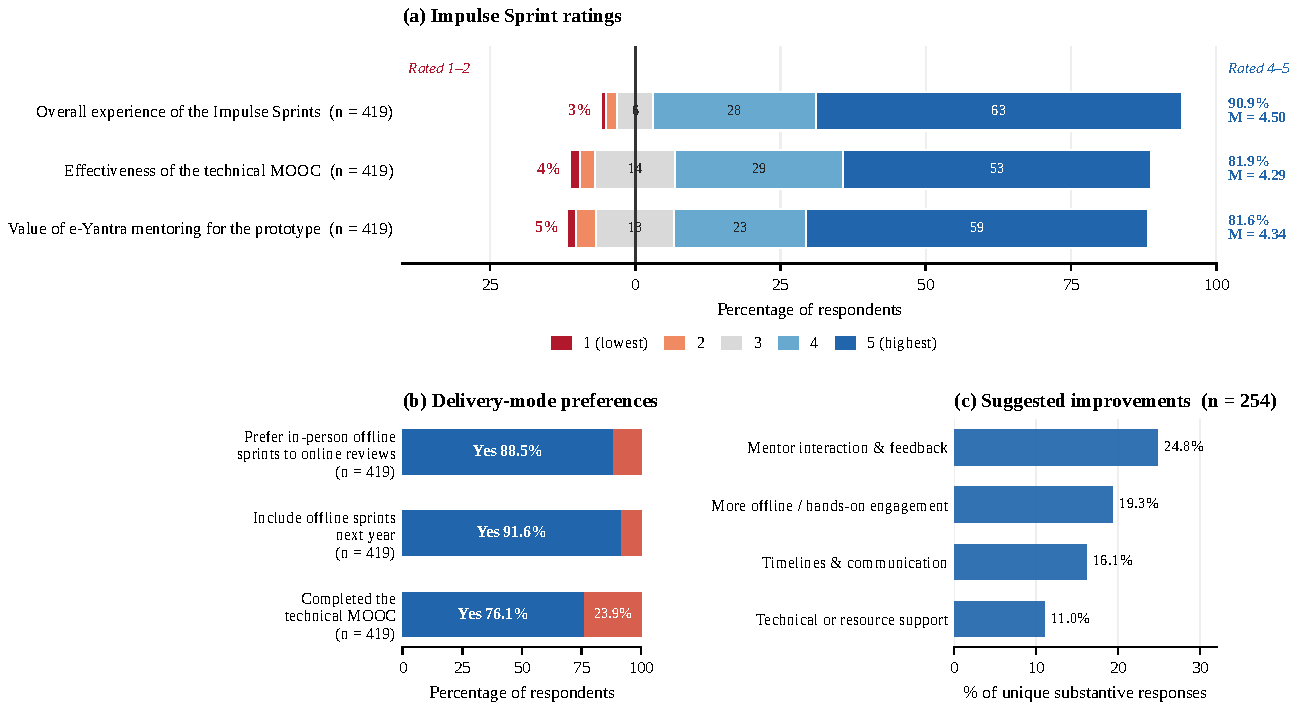
\includegraphics[width=\textwidth]{figures/image5}
\caption{Impulse Sprint feedback (n = 419). (a) Ratings of the Impulse Sprint experience, the technical MOOC, and mentoring; values on the right give the percentage rating 4–5 and the mean (M). (b) Delivery-mode preferences and technical MOOC completion. (c) Themes in 254 unique substantive improvement suggestions (multi-label coding).}
\label{fig5}
\end{figure}

However, the improvement suggestions demonstrate that participants wanted more of these forms of support rather than a fundamentally different model. Among 254 unique substantive Impulse Sprint improvement responses, mentor interaction and feedback was the most frequent recurring theme (24.8\%), followed by requests for more offline or hands-on engagement (19.3\%), improvements to timelines and communication (16.1\%), and stronger technical or resource support (11.0\%) (Fig.~\ref{fig5}c). This pattern suggests that the value of the sprint was closely connected to opportunities for situated feedback while teams were actively making. Participants asked for more regular mentor interaction, doubt-clearing opportunities, practical sessions, and quicker feedback rather than additional abstract instruction. One participant, for example, suggested that eYIC could improve support through \emph{“more hands-on sessions, beginner-friendly guidance, regular doubt-clearing interactions, and better communication about resources, timelines, and opportunities.”}

The end-of-programme reflections reinforce this interpretation. Among 167 unique substantive responses describing the most valuable part of eYIC, nearly half referred to hands-on or end-to-end project learning (46.1\%). Problem and stakeholder understanding appeared in 44.3\% of responses, while technical skill development appeared in 31.7\% and teamwork or collaboration in 28.7\%. Mentor, jury, or expert feedback was mentioned in 16.8\%, and presentation, communication, or confidence development appeared in 15.6\%. Responses could contain multiple themes and were therefore coded into more than one category.

A participant summarised the experience as:\emph{“The most valuable part was the hands-on learning experience-working on a complete problem lifecycle from ideation to implementation.”} Another participant described the programme as teaching them \emph{“how to solve a problem right from defining it to developing [it] to making it market ready.”} Such reflections suggest that the educational value of eYIC was perceived not as mastery of one particular technology but as experience of an extended innovation trajectory, involving problem framing, technical learning, collaboration, prototyping, feedback, and communication.

Self-paced learning resources were intended to provide foundational technical knowledge alongside project development. The programme offered courses in areas including embedded systems, software foundations, ROS, IoT, and drone technology, while innovation and entrepreneurship content accompanied the earlier ideation phase. Participant feedback indicated generally positive perceptions of the learning resources. However, the programme team identified a major implementation issue: many teams were not sufficiently aware of the technical MOOCs available to them. This suggests that providing self-paced resources was not in itself sufficient to ensure their use. Their value depended on how visibly they were introduced and how closely they were connected to immediate project needs and sprint milestones. For future iterations, the programme therefore requires stronger onboarding and more explicit integration of learning resources into the developmental trajectory of teams.

\subsection{Implementation Emerged as the Critical Point of Difficulty}

The clearest finding from the end-of-programme survey concerns where participants experienced the greatest difficulty. When 202 respondents were asked to identify the most challenging stage of their journey, 126 participants (62.4\%) selected Implementation. Submission was a distant second at 18.3\%, followed by Ideation at 11.4\%, Proposal development at 3.5\%, and Other challenges at 4.5\% (Fig.~\ref{fig6}a). This distribution indicates that the central difficulty did not lie primarily in generating ideas. Instead, challenges became most acute when teams had to translate ideas into functioning systems. The corresponding open-ended descriptions explain what “implementation” involved for participants. Exploratory coding of 164 unique substantive challenge descriptions showed that technical implementation, integration, prototyping, testing, or debugging appeared in approximately 47.0\% of responses. Time constraints, deadlines, examinations, and balancing eYIC with academic commitments appeared in 39.6\%. Other recurring challenges included unfamiliar technologies or learning curves (12.8\%), obtaining data or undertaking field and stakeholder validation (12.2\%), and team coordination (10.4\%) (Fig.~\ref{fig6}b).A participant described the difficulty as: \emph{“The biggest challenge was integrating different components-both hardware and software-into a stable and reliable system.”} Another explained that the difficulty was the gap between \emph{“theoretical understanding and practical implementation,”} particularly when integrating hardware, software, and data processing. These comments point towards a critical transition in the learning trajectory: understanding what should be built was different from developing a reliable working system under real constraints.

\begin{figure}[htbp]
\centering
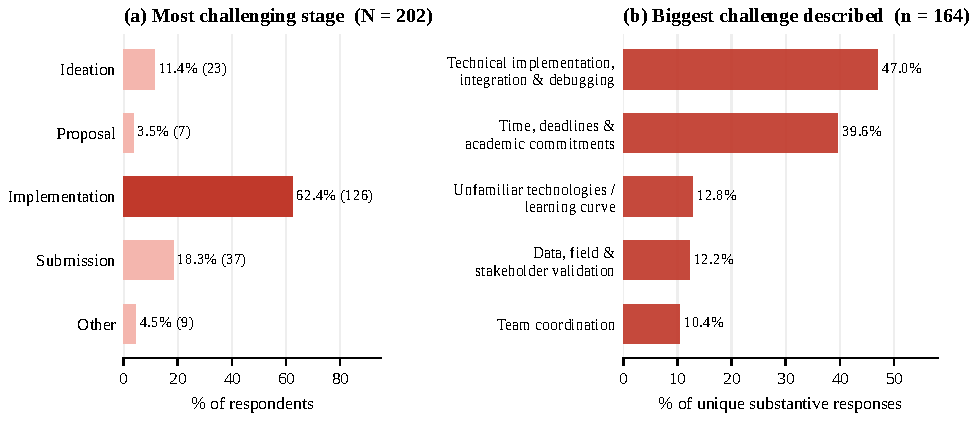
\includegraphics[width=\textwidth]{figures/image6}
\caption{Implementation as the critical point of difficulty. (a) Stage identified as most challenging (N = 202). (b) Themes in 164 unique substantive descriptions of the biggest challenge (multi-label coding; percentages do not sum to 100).}
\label{fig6}
\end{figure}

Time intensified this difficulty. Participants described balancing academic schedules, examinations, commuting, college hours, and project deadlines. In several responses, implementation challenges were not attributed purely to lack of technical competence but to the combination of technical uncertainty and temporal pressure. The finding therefore suggests a shift in the locus of scaffolding required across the programme. During early stages, participants benefited primarily from support in defining problems and organising their thinking. During implementation, they required more specialised technical guidance, debugging support, resources, sustained mentorship, and time to iterate.

\subsection{Mentorship Was Valued, but Continuity and Domain Fit Were Uneven}

Mentorship emerged throughout the dataset as both one of eYIC's strongest supports and one of its recurring implementation tensions. At the end of the programme, 185 of 202 respondents (91.6\%) answered positively to the mentor-related yes/no item in the feedback form, compared with 81.6\% of Impulse Sprint respondents who rated mentoring 4 or 5 and 77.2\% of Regional Finale respondents who rated mentors 3 or 4 on a four-point scale (Fig.~\ref{fig7}a). The broader qualitative data also contain repeated references to the value of mentor, jury, and expert feedback. Participants described mentors as helping them reconsider technical decisions, understand real-world limitations, and receive perspectives unavailable within their own institutions. However, the explanations provided by the smaller group who reported inadequate guidance (n = 12) reveal several issues (Fig.~\ref{fig7}c). Participants referred to difficulty contacting mentors after sprint interactions, mentors changing between stages, lack of domain-specific expertise, limited follow-up, and interactions that felt more evaluative than developmental. One participant wrote:\emph{“Mentors were different for each impulse sprint; because of that we found it difficult to convey the solution to mentors.”} Another commented: \emph{“I think that the mentors could have been more interactive than just evaluating us during the sprints.”}

\begin{figure}[htbp]
\centering
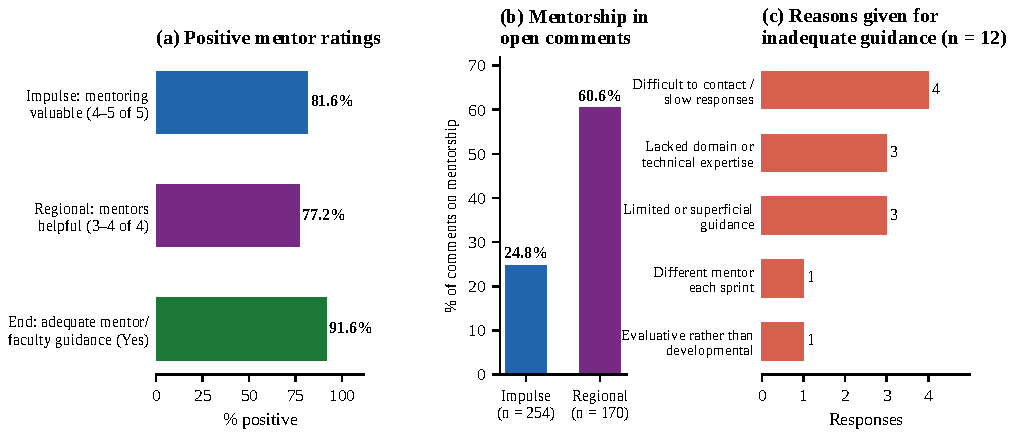
\includegraphics[width=\textwidth]{figures/image7}
\caption{Mentorship across stages. (a) Share of positive mentor-related responses at each stage; scales differ by stage, as labelled. (b) Share of open comments mentioning mentorship or feedback at the Impulse Sprint and Regional Finale stages. (c) Reasons given by respondents who reported inadequate guidance (n = 12 substantive explanations).}
\label{fig7}
\end{figure}

These responses reveal an important distinction between periodic expert evaluation and sustained mentoring. A mentor who meets a team briefly can provide useful critique, but teams working through complex implementation problems may require continuity so that the mentor understands the history of the project, earlier design decisions, and unresolved technical difficulties. This tension becomes even more prominent in the regional-stage feedback. Among 170 unique substantive comments, mentorship or feedback appeared in approximately 60.6\% (Fig.~\ref{fig7}b), making it the most frequent theme. Participants often requested dedicated mentors, recurring check-ins, stronger domain matching, and opportunities to discuss problems between formal evaluation milestones.

Thus, the findings do not indicate that mentorship was ineffective. Rather, they suggest that its perceived value created greater expectations for continuity, accessibility, and disciplinary fit, which became increasingly difficult to provide consistently as the programme operated at national scale. These concerns were also recognised by the programme team, which subsequently proposed more systematic mentor training, clearer alignment around evaluation expectations, and regular review cycles to provide greater continuity of support.

\subsection{Later-Stage Participants Required More Specialised and Context-Sensitive Support}

The regional-stage feedback reveals how participant needs changed as projects became more technically mature. After removing duplicate respondent records, 189 unique responses were retained from this stage. The overall-experience item showed strong positive perception, with a mean of 4.46/5 and 88.9\% selecting 4 or 5. On the four-point items, sprint structure and clarity of objectives were rated highly, with 89.4\% and 88.9\% of respondents selecting 3 or 4, whereas sprint timelines and implementing the project as planned drew the largest shares of low ratings, at 24\% and 25\% respectively (Fig.~\ref{fig8}a). Open-ended responses became substantially more specific about the conditions necessary to advance projects further. Among 170 unique substantive comments, the most visible recurring themes were mentorship and feedback (60.6\%), technical or prototype-related support (44.7\%), and timeline or deadline pressure (41.2\%). Participants also raised the need for stronger access to industry, domain experts, farmers, or other stakeholders (28.2\%); clearer evaluation and judging criteria (27.6\%); and greater regional or travel accessibility (18.2\%) (Fig.~\ref{fig8}b).

\begin{figure}[htbp]
\centering
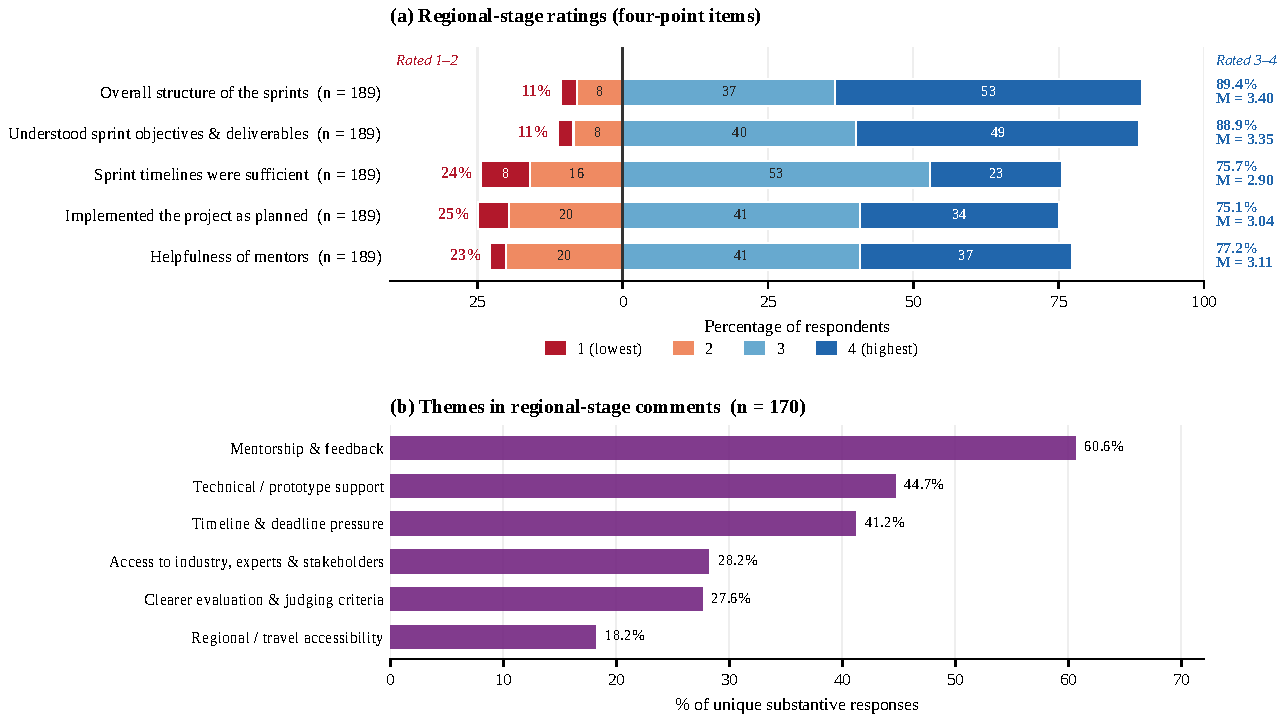
\includegraphics[width=\textwidth]{figures/image8}
\caption{Later-stage needs. (a) Regional-stage ratings on four-point items (n = 189 unique respondents); values on the right give the percentage rating 3–4 and the mean (M). (b) Themes in 170 unique substantive regional-stage comments (multi-label coding).}
\label{fig8}
\end{figure}

This differs considerably from the early-stage feedback. At the beginning of the programme, participants valued frameworks that helped them think about innovation. By the regional stages, teams were asking for domain expertise, specialised technical troubleshooting, clearer evaluation standards, resources, and access to stakeholders. Participants also questioned whether different types of solutions should always be assessed through identical criteria. Some software-oriented teams, for example, raised concerns about being compared directly with hardware-heavy solutions. Others requested that evaluation rubrics and judging parameters be communicated earlier so that teams understood the dimensions against which their progress would be judged. Participants’ concerns related not only to knowing the evaluation criteria in advance but also to whether common criteria adequately represented heterogeneous project forms. Requests therefore concerned both transparency-through advance rubrics, templates, and sample submissions-and differentiation where software-oriented, hardware-intensive, or domain-specific projects followed substantially different developmental trajectories.

These responses suggest that as projects diversify and mature, a generic support structure becomes increasingly difficult to sustain. The programme must simultaneously accommodate differences in technological complexity, disciplinary background, access to resources, domain requirements, and project trajectories. Participants also raised geographical and scheduling constraints, including travel to regional venues, conflicts with examinations and academic calendars, and limited opportunities to attend in-person workshops. Requests for more geographically distributed centres therefore reflected a tension between the perceived value of face-to-face engagement and the difficulty of providing such experiences equitably at national scale.

\subsection{A Cross-Stage Shift in the Nature of Scaffolding}

Across the datasets, a broader developmental pattern emerged. Participants did not require the same type of support throughout the six-month innovation journey. While ideation, the most valued support helped participants identify problems, understand user needs, structure ideas, and think about innovation and entrepreneurship systematically. For prototype development, the emphasis shifted towards hands-on building, mentor interaction, technical feedback, and opportunities to troubleshoot evolving artefacts. During implementation, technical integration, debugging, learning unfamiliar technologies, and managing time alongside academic demands became the dominant challenges. By the regional and final stages, participants increasingly required specialised mentorship, domain expertise, stakeholder access, transparent evaluation, logistical support, and sufficient time for refinement.The progression can therefore be understood as a movement from conceptual scaffolding to developmental scaffolding to technical and contextual scaffolding. This shift represents an important insight from the eYIC experience. Providing a sequence of milestones alone is not sufficient for supporting open-ended innovation at scale. The nature of support itself needs to evolve as teams move from understanding a problem to producing, validating, and communicating a working solution. At the same time, end-of-programme reflections suggest that it was precisely this extended journey that participants valued. Participants repeatedly described gaining experience in problem identification, stakeholder interaction, technical implementation, teamwork, troubleshooting, presentation, and learning under constraints. Rather than identifying a single workshop, MOOC, or competition event as the source of learning, their reflections frequently described the entire trajectory from idea to implementation as the key educational experience.

\section{Reflections from the Orchestration Team}

Implementing eYIC as a six-month, national innovation programme generated a set of design and orchestration lessons that extend beyond the participant outcomes reported in the previous section. From the orchestration team’s perspective, the central challenge was not simply to provide students with a sequence of activities, but to sustain appropriate forms of support as teams moved from loosely framed ideas towards increasingly complex and heterogeneous solutions. Several tensions became visible during implementation, particularly around open-ended problem finding, time, mentoring, resource integration, and programme scale.

\subsection{Open-Ended Problem Finding Requires Structured Entry Points}

One of the distinguishing features of eYIC was that teams were encouraged to begin with problems from real contexts rather than being assigned predefined technical tasks. The orchestration team regarded this openness as pedagogically important because it created space for students to investigate needs, engage stakeholders, and determine what kinds of technological responses might be appropriate. At the same time, it was also one of the most difficult elements to implement. Teams sometimes entered the programme with a technology they already wished to use and subsequently searched for a problem that could justify that technology. Access to agricultural settings and relevant stakeholders was also uneven, and the use of a single broad thematic domain sometimes resulted in similar problem formulations emerging across teams.

The experience therefore suggests that open-endedness and structure should not be treated as opposites. Completely prescribing problems would undermine an important aspect of the programme, while leaving teams without sufficient entry points can make authentic problem finding difficult, particularly for students with limited prior exposure to the domain. Curated problem spaces, stakeholder access, exemplar cases, and guided field-engagement opportunities may provide enough structure to help teams begin inquiry without converting the programme into a prescribed problem-solving competition. Open-ended problem finding also created consequences for evaluation. As teams developed solutions, project forms became increasingly diverse, ranging from software-oriented systems to hardware-intensive prototypes. Applying identical evaluation expectations across these different trajectories was not always straightforward. The orchestration team therefore recognised that openness in problem selection needs to be accompanied by evaluation mechanisms capable of recognising variation in how different types of solutions develop and demonstrate progress.

\subsection{The Stage Requiring the Most Iteration Also Requires the Most Time}

The programme schedule was necessarily organised around common milestones so that hundreds of participants, reviewers, and regional partners could progress through the challenge in a coordinated manner. However, implementation revealed a tension between the administrative logic of milestones and the learning logic of iterative development. The implementation stage required teams to integrate components, test assumptions, encounter failures, troubleshoot systems, and repeatedly revise their prototypes. Yet this was also the stage in which the programme placed increasingly demanding expectations on participants within relatively compressed timelines. The requirement to demonstrate a working prototype provided an important developmental target, but it also concentrated technical work during a period when many students were simultaneously managing examinations, classes, commuting, and other academic responsibilities. The orchestration team therefore came to view time not simply as a scheduling issue but as a pedagogical resource. Iterative innovation requires room for unsuccessful attempts, redesign, and repeated testing. Future programme designs should consequently allocate time according to the nature of the work expected at different stages rather than distributing time primarily according to administrative convenience. In particular, implementation may require longer intervals between major reviews than ideation or proposal development.

\subsection{Periodic Review and Sustained Mentorship Are Different Support Structures}

The programme demonstrated the value of expert interaction, but it also led the orchestration team to reconsider how the term mentorship was being used. Much of what teams experienced as mentoring consisted of scheduled sprint reviews in which programme staff or experts examined progress and provided feedback. These interactions were valuable, but reviewers could change between stages, individual sessions were relatively short, and teams did not necessarily have access to the same person between formal reviews. There was no formal programme-wide mechanism that ensured an ongoing mentor remained with a team across the complete project trajectory.

This distinction became particularly important during implementation. A reviewer can identify weaknesses in a prototype during a single interaction, whereas an ongoing mentor can accumulate knowledge of the team’s earlier decisions, constraints, failed attempts, and unresolved questions. The latter becomes increasingly valuable as projects become technically and contextually complex. The experience therefore suggests that expert review and mentoring should be deliberately designed as complementary rather than interchangeable structures. Reviews can provide milestone-based critique and ensure common standards, while sustained mentors can support developmental continuity between those milestones. Establishing such a model at scale would require explicit mentor roles, clearer expectations, appropriate mentor-team matching, and mechanisms for monitoring mentor engagement rather than assuming that mentoring will emerge naturally from occasional interactions.

\subsection{Resources Must Be Integrated into the Learning Journey, Not Merely Made Available}

A similar lesson emerged from the programme’s technical learning resources. The MOOCs were intended to provide foundational knowledge that participants could draw upon while developing their solutions. However, the orchestration team observed that awareness and use of these resources were weaker than intended. The courses were deliberately kept low-pressure: they carried no certification, had limited connection to evaluation, did not operate through strongly enforced deadlines, and participation was not systematically tracked. Individually, these design choices were intended to preserve flexibility; collectively, they reduced the visibility and immediacy of the resources for participating teams. This led to an important distinction for programme design: making a resource available is different from embedding that resource in the programme.

Self-paced materials are more likely to become meaningful when participants encounter them at the point at which the corresponding knowledge becomes necessary. Technical modules could therefore be aligned explicitly with sprint milestones, referenced during mentor interactions, or connected with project tasks that require teams to apply particular concepts. The same lesson applied more broadly to programme communication. Although instructions and resources were available through programme channels, teams continued to request clarification at different stages. From the orchestration perspective, information that is technically available may still be functionally inaccessible if participants do not encounter it when it becomes relevant. Important expectations therefore need to be communicated repeatedly, through multiple channels, and at the point of need.

\subsection{Scaling Personalised Innovation Support Produces Orchestration Trade-Offs}

The 2025–26 edition demonstrated that an extended hybrid innovation programme could be coordinated across a geographically distributed participant population. Regional partner institutions enabled workshops and offline sprints to be organised closer to participating teams, while online components made periodic interaction possible across locations. The programme was also able to modify aspects of implementation during the cycle when emerging needs became visible. However, the components most valued within such a model like individual reviews, personalised feedback, technical troubleshooting, and in-person engagement, were also among the most labour-intensive to provide. These activities depended heavily on a relatively small orchestration team that was simultaneously responsible for venues, communication, reimbursements, certificates, reviews, and participant coordination. This suggests that scaling cannot be understood simply as increasing participant numbers. Sustaining quality at a larger scale requires distributing expertise and responsibility across mentors, regional hosts, participating institutions, and other partners.

Regionalisation itself introduced another tension. Partner institutions made nationwide in-person engagement possible, but differences in local infrastructure, resources, and implementation practices could also create different participant experiences across locations. Clear host expectations, shared operating procedures, and consistent support therefore become increasingly important as delivery is distributed across multiple centres. A related tension emerged between consistency and flexibility. Common rules for attendance, scheduling, submissions, and progression made national coordination possible and provided a shared structure for participants. At the same time, students belonged to institutions with different examination schedules, working days, academic calendars, and local constraints. Uniformity therefore supported fairness and manageability but could also limit participation for particular groups. The challenge for future iterations is not to choose between consistency and flexibility, but to identify which elements must remain standardised and where controlled flexibility can be introduced without compromising programme coherence.

\subsection{Support during Uncertainty Is Different from Rewarding Later Success}

The programme provided material forms of support such as travel assistance, component reimbursement, recognition, and awards. These mechanisms enabled teams that progressed to later stages to build and demonstrate physical prototypes and participate in in-person events. However, much of this assistance became available after teams had already demonstrated substantial progress.From the orchestration team's perspective, this highlighted a distinction between rewarding progress and sustaining participation. Teams may require support most intensely during the earlier and middle stages, when the feasibility of their idea remains uncertain, technical pathways are unclear, and commitment is still developing. Future models could therefore consider whether smaller forms of technical, material, or mentoring support should be introduced earlier rather than concentrating most resources near the final stages.

This issue is particularly relevant because the programme was open across degree levels while many participants were still relatively early in their studies. Expectations such as producing integrated prototypes and presenting solutions in an incubator-oriented setting were intentionally ambitious, but the experience suggested that ambitious outcomes need to be accompanied by scaffolding appropriate to the experience level of the participating cohort. The lesson is therefore not to lower expectations, but to prepare mentors, reviewers, resources, and timelines around the students who actually participate.

\subsection{Reconsidering the Purpose of the eYIC}

A final reflection concerned the programme's broader purpose. eYIC had historically been framed partly around supporting student entrepreneurship and accelerating promising projects towards startup formation. Consequently, later stages included product demonstrations and pitching to potential incubators. The participant's experience, however, suggested that much of the perceived value lay in the journey itself, learning to frame problems, work with constraints, move from ideas towards functioning systems, and experience an extended project lifecycle.

This led the orchestration team to reconsider startup creation as one possible outcome rather than the primary measure of programme success. A more appropriate framing may be that eYIC seeks to cultivate an innovative and entrepreneurial way of approaching problems. Some teams may subsequently pursue incubation or venture creation; others may carry the capacities developed through the programme into further study, employment, research, or future projects. From this perspective, the value of the challenge lies not only in the quality of the final prototype but also in enabling students to experience the uncertainty and iteration involved in taking an idea seriously enough to investigate, build, test, defend, and revise it.

Taken together, the 2025-26 eYIC experience suggests that supporting innovation at scale involves more than assembling workshops, MOOCs, mentoring, evaluation, and competition milestones. These components need to be orchestrated differently as projects mature. Open-ended problem finding requires structured entry points; implementation requires time for iteration; periodic review should be complemented by sustained mentorship; learning resources must be connected to moments of use; and scaling personalised support requires distributed responsibility across institutions and partners.

The central orchestration lesson is therefore that the programme cannot scale simply by reproducing the same support structures for a larger number of teams. As participants move from problem identification towards implementation and deployment, their needs become increasingly differentiated and resource-intensive. Future iterations of eYIC must therefore balance openness with structure, consistency with flexibility, ambition with participant readiness, and national reach with the personalised support required for meaningful innovation learning.

\section{Discussion}

The eYIC experience suggests that a large-scale innovation challenge can function as an extended learning environment rather than only as a competition. Across the programme, teams moved from problem identification and ideation to prototyping, troubleshooting, validation, and communication. Participant reflections indicate that the value of the programme lies less in any single workshop or final event and more in experiencing the complete trajectory from identifying a problem to developing and communicating a working solution. This aligns with experiential and project-based learning perspectives, where learning develops through sustained cycles of action, reflection, experimentation, and artefact development

\subsection{Scaffolding Needs Changed across the Innovation Journey}

A central finding is that teams did not require the same kind of support throughout the programme. Early-stage participants valued support for problem identification, user understanding, ideation, and structuring their thinking. During prototype development, hands-on engagement, technical feedback, troubleshooting, and mentor interaction became more important. By later stages, teams increasingly sought specialised technical expertise, stakeholder access, clearer evaluation criteria, logistical support, and additional time for refinement. This progression can be understood as a movement from conceptual scaffolding, to developmental scaffolding, and finally to technical and contextual scaffolding. Cognitive apprenticeship \cite{b36} helps explain this transition: initial modelling and guidance can introduce processes such as problem framing, while later stages require coaching, feedback, reflection, and support around participants’ own evolving artefacts. The implication is that innovation programmes should not only provide milestones; the support associated with those milestones must also change as projects mature.

\subsection{Open-Ended Innovation Requires Structure, Time, and Sustained Guidance}

eYIC differed from competitions based on predefined technical tasks by asking teams to identify problems within a broad societal domain. This openness encouraged problem-first thinking but also created difficulties. Some teams began with technologies they wanted to use and searched for suitable problems, while stakeholder access was uneven and heterogeneous project types created challenges for common evaluation criteria. Thus, open-endedness does not imply the absence of structure. Curated problem spaces, access to stakeholders, exemplar cases, and differentiated evaluation criteria may help preserve student agency while providing stronger entry points. The implementation stage further revealed that innovation requires sufficient time for testing, failure, and redesign. Participants identified implementation as the most difficult stage, particularly because technical integration and debugging coincided with academic workload and programme deadlines. From the orchestration perspective, the stage requiring the most iteration was also one of the most temporally compressed. This suggests that time should be treated as a pedagogical resource rather than only as a scheduling constraint. The same principle applies to mentorship. Although expert feedback was valued, much of the support functioned as periodic sprint review rather than sustained mentoring. Reviewers could change across stages, interactions were short, and there was no formal mechanism ensuring continuity with the same mentor. Future designs should therefore distinguish expert review, which supports milestone-based evaluation, from ongoing mentorship, which provides continuity across the project lifecycle.

\subsection{Hybrid and Resource-Rich Designs Need Purposeful Integration}

The strong preference for offline sprints suggests that online and in-person formats served different functions. Online components enabled geographically distributed participation, while in-person settings supported rapid troubleshooting, richer mentor interaction, peer engagement, and hands-on work. At the same time, increasing offline activity creates challenges around travel, regional infrastructure, and equitable access. A purposeful hybrid model may therefore use online delivery for learning resources and routine reviews, while reserving in-person activity for stages where co-presence adds particular value, such as prototype development and intensive feedback. The experience with technical MOOCs provides a related lesson. Although resources were available, many teams were not sufficiently aware of or engaged with them. The courses were weakly connected to deadlines, evaluation, certification, and tracked progress, reducing their visibility within the programme. This suggests that availability of a resource does not automatically make it a scaffold. Learning resources become more meaningful when they are explicitly connected to the project stage in which participants need them

\subsection{Scaling Innovation Education Is an Orchestration Challenge}

The programme demonstrated that a multi-stage hybrid innovation challenge could be implemented across a large number of institutions, including institutions beyond the existing e-Yantra network. However, the most valued elements such as individual feedback, mentor interaction, technical troubleshooting, and offline engagement, were also the most resource-intensive. Regional delivery additionally created variation in participant experience, while uniform programme rules sometimes conflicted with different academic calendars and local circumstances. Scaling such programmes therefore involves more than increasing participant numbers. It requires distributing responsibility across mentors, regional hosts, participating institutions, and domain partners while maintaining sufficient consistency in learning expectations and evaluation. Some elements may need to remain standardised, while others such as mentoring, scheduling, technical support, and regional implementation may require controlled flexibility.

Finally, the experience invites reconsideration of programme outcomes. Although eYIC included startup acceleration and incubator-oriented pitching, participants placed greater value on problem framing, iterative development, technical learning, collaboration, and experiencing the complete idea-to-solution journey. Startup formation may therefore be understood as one possible outcome rather than the sole endpoint. More broadly, eYIC can be viewed as an innovation-learning pathway in which competition provides structure and motivation while the educational value emerges from sustained engagement with authentic problems.

\begin{thebibliography}{99}

\bibitem{b1}
Abelha, M., Fernandes, S., Mesquita, D., Seabra, F., Ferreira-Oliveira, A.T.: Graduate employability and competence development in higher education—a systematic literature review using PRISMA. Sustainability \textbf{12}(15), 5900 (2020)

\bibitem{b2}
Tushar, H., Sooraksa, N.: Global employability skills in the 21st century workplace: a semi-systematic literature review. Heliyon \textbf{9}(11) (2023)

\bibitem{b3}
Oliver, B.: Redefining graduate employability and work-integrated learning: proposals for effective higher education in disrupted economies. J. Teach. Learn. Grad. Employability \textbf{6}(1), 56–65 (2015)

\bibitem{b4}
Kolb, D.A.: Experiential Learning: Experience as the Source of Learning and Development, 2nd edn. Pearson Education, Upper Saddle River (2015)

\bibitem{b5}
Kolb, A.Y., Kolb, D.A.: Learning styles and learning spaces: enhancing experiential learning in higher education. Acad. Manage. Learn. Educ. \textbf{4}(2), 193–212 (2005)

\bibitem{b6}
Chen, C.H., Yang, Y.C.: Revisiting the effects of project-based learning on students' academic achievement: a meta-analysis investigating moderators. Educ. Res. Rev. \textbf{26}, 71–81 (2019)

\bibitem{b7}
Kokotsaki, D., Menzies, V., Wiggins, A.: Project-based learning: a review of the literature. Improving Schools \textbf{19}(3), 267–277 (2016)

\bibitem{b8}
Almulla, M.A.: The effectiveness of the project-based learning (PBL) approach as a way to engage students in learning. SAGE Open \textbf{10}(3) (2020)

\bibitem{b9}
Razzouk, R., Shute, V.: What is design thinking and why is it important? Rev. Educ. Res. \textbf{82}(3), 330–348 (2012)

\bibitem{b10}
Brown, T.: Design thinking. Harvard Bus. Rev. \textbf{86}(6), 84–92 (2008)

\bibitem{b11}
Micheli, P., Wilner, S.J.S., Bhatti, S.H., Mura, M., Beverland, M.B.: Doing design thinking: conceptual review, synthesis, and research agenda. J. Prod. Innov. Manage. \textbf{36}(2), 124–148 (2019)

\bibitem{b12}
St-Jean, É., Audet, J.: The role of mentoring in the learning development of the novice entrepreneur. Int. Entrep. Manage. J. \textbf{8}, 119–140 (2012)

\bibitem{b13}
Spelt, E.J.H., Biemans, H.J.A., Tobi, H., Luning, P.A., Mulder, M.: Teaching and learning in interdisciplinary higher education: a systematic review. Educ. Psychol. Rev. \textbf{21}(4), 365–378 (2009)

\bibitem{b14}
Dewey, J.: Experience and Education. Macmillan, New York (1938)

\bibitem{b15}
Blumenfeld, P.C., Soloway, E., Marx, R.W., Krajcik, J.S., Guzdial, M., Palincsar, A.: Motivating project-based learning: sustaining the doing, supporting the learning. Educ. Psychol. 26(3–4), 369–398 (1991)

\bibitem{b16}
Strobel, J., van Barneveld, A.: When is PBL more effective? A meta-synthesis of meta-analyses comparing PBL to conventional classrooms. Interdiscip. J. Probl.-Based Learn. 3(1), 44–58 (2009)

\bibitem{b17}
Chen, J., Kolmos, A., Du, X.: Forms of implementation and challenges of PBL in engineering education: a review of literature. Eur. J. Eng. Educ. 46(1), 90–115 (2021)

\bibitem{b18}
Guo, P., Saab, N., Post, L.S., Admiraal, W.: A review of project-based learning in higher education: student outcomes and measures. Int. J. Educ. Res. 102, 101586 (2020)

\bibitem{b19}
Oyetade, K., Zuva, T., Harmse, A.: Evaluation of the impact of hackathons in education. Cogent Educ. 11(1), 2392420 (2024)

\bibitem{b20}
Nandi, A., Mandernach, M.: Hackathons as an informal learning platform. In: Proceedings of the 47th ACM Technical Symposium on Computing Science Education (SIGCSE), pp. 346–351. ACM (2016)

\bibitem{b21}
Sotaquirá-Gutiérrez, R., Beltran, L.M., Garzon Ruiz, J.P.: Hackathons as experiential learning platforms for engineering design skills. Cogent Educ. 12(1), 2442187 (2025)

\bibitem{b22}
Hamilton, L.K., Boman, J., Rubin, H., Sahota, B.K.: Examining the impact of a university mentorship program on student outcomes. Int. J. Mentor. Coach. Educ. 8(1), 19–36 (2019)

\bibitem{b23}
Nabi, G., Walmsley, A., Mir, M., Osman, S.: The impact of mentoring in higher education on student career development: a systematic review and research agenda. Stud. High. Educ. 50(4), 739–755 (2025)

\bibitem{b24}
Hone, K.S., El Said, G.R.: Exploring the factors affecting MOOC retention: a survey study. Comput. Educ. 98, 157–168 (2016)

\bibitem{b25}
Israel, M.J.: Effectiveness of integrating MOOCs in traditional classrooms for undergraduate students. Int. Rev. Res. Open Distrib. Learn. 16(5), 102–118 (2015)

\bibitem{b26}
Ivanitskaya, L., Clark, D., Montgomery, G., Primeau, R.: Interdisciplinary learning: process and outcomes. Innov. High. Educ. 27(2), 95–111 (2002)

\bibitem{b27}
Blom, A., Saeki, H.: Employability and skill set of newly graduated engineers in India. Policy Research Working Paper 5640, World Bank, Washington, DC (2011)

\bibitem{b28}
Aspiring Minds: National Employability Report for Engineers. Aspiring Minds, Gurgaon (2019)

\bibitem{b29}
Ministry of Human Resource Development: National Education Policy 2020. Government of India, New Delhi (2020)

\bibitem{b30}
Krithivasan, S., Shandilya, S., Arya, K., Lala, K., Manavar, P., Patil, S., Jain, S.: Learning by competing and competing by learning: experience from the e-Yantra Robotics Competition. In: 2014 IEEE Frontiers in Education Conference (FIE) Proceedings, pp. 1–8. IEEE (2014)

\bibitem{b31}
Krithivasan, S., Shandilya, S., Lala, K., Arya, K.: Massive project based learning through a competition: impact of and insights from the e-Yantra Robotics Competition (eYRC–2013). In: 2014 IEEE Sixth International Conference on Technology for Education (T4E), pp. 156–163. IEEE (2014). \url{https://doi.org/10.1109/T4E.2014.13}

\bibitem{b32}
Krithivasan, S., Shandilya, S., Shakya, S., Arya, K., Lala, K.: Building inclusiveness in a PBL based online robotics competition: challenges and outcomes. In: 2016 International Conference on Learning and Teaching in Computing and Engineering (LaTICE), pp. 9–13. IEEE (2016)

\bibitem{b33}
Karia, K., Bessariya, R., Lala, K., Arya, K.: Learning while competing – 3D modeling \& design. arXiv:1905.07644 (2019)

\bibitem{b34}
Jadhav, S., Karia, K., Trimukhe, P., Jena, S., Arya, K.: PBL approach in online robotics competition in resource-poor environments: Maze Solver Robot. In: 2021 IEEE Global Engineering Education Conference (EDUCON), pp. 492–498. IEEE (2021)

\bibitem{b35}
Brown, J.S., Collins, A., Duguid, P.: Situated cognition and the culture of learning. Educ. Res. \textbf{18}(1), 32–42 (1989)

\bibitem{b36}
Collins, A., Brown, J.S., Newman, S.E.: Cognitive apprenticeship: teaching the crafts of reading, writing, and mathematics. In: Resnick, L.B. (ed.) Knowing, Learning, and Instruction: Essays in Honor of Robert Glaser, pp. 453–494. Lawrence Erlbaum Associates, Hillsdale (1989)

\bibitem{b37}
Johnson, D.W., Johnson, R.T.: An educational psychology success story: social interdependence theory and cooperative learning. Educ. Res. \textbf{38}(5), 365–379 (2009)

\end{thebibliography}

\end{document}
